\documentclass[tikz]{standalone}
\usepackage{tikz}
\usetikzlibrary{arrows}

\begin{document}

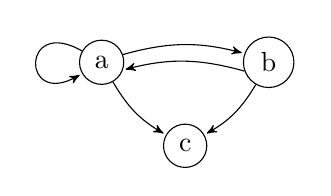
\begin{tikzpicture}[->,>=stealth',shorten >=1pt,auto,node distance=1.5cm,
main node/.style={circle, draw}]


 			\node[main node] (c) {c};
			\node[main node] (b) [above right of=c] {b};
			\node[main node] (a) [above left of=c] {a};


                \useasboundingbox (c) rectangle (-2,1.5) --
                (c) rectangle (1.5,1.5);

		\path[every node/.style={font=\sffamily\small}]
				(a.20) edge [bend left=15] (b.160)
				(b.-160) edge [bend right=15] (a.-20) 
				(a) edge [bend right=15] (c)
				(b) edge [bend left=15] (c)
				(a) edge [out = 150, in = 210, loop] (a);
				
	

\end{tikzpicture}

\end{document}


%%% Local Variables: 
%%% mode: latex
%%% TeX-master: t
%%% End: 
